% BangorEE - (an unofficial) Electronic Engineering Dissertation LaTeX Class.
% Usage info and bug reports at https://github.com/owenjones/bangoree

\documentclass[msc]{bangoree}

\usepackage{lipsum} % To create some filler content
\usepackage[style=authoryear-ibid]{biblatex}
\usepackage{amsmath}
\usepackage{subcaption}
\usepackage{appendix}

\title{Leksis: Prawf Geirfa Ymaddasol Am Ieithoedd Isadnodd}
\author{Alan Kersaudy}
\course{Technoleg Iaith}
\date{Medi, 2025}
\supervisor{Dr.\ G. Bovolenta}

\addbibresource{references.bib}

\renewcommand{\contentsname}{Cynnwys}
\renewcommand{\listfigurename}{Rhestr o Ffigurau}
\renewcommand{\listtablename}{Rhestr o Dablau}
\renewcommand{\nomname}{Rhestr o Dalfyriadau}
\renewcommand{\appendixname}{Atodiad}
\makeatletter
\renewcommand{\@chapapp}{Pennod}
\makeatother

\begin{document}
    \maketitle
    \statements
    \abstract{abc}
    \acknowledgements{\lipsum[1]}
    \tables
    
    \content
    \chapter{Cyflwyniad}    
    \abbrv{IIA}{Iaith (neu Ieithoedd) Isadnodd}
Mae'r bennod gyntaf hon yn cyflwyno'r cyd-destun, cwmpas a phwrpas y traethawd hir hwn. Yn benodol, daw'r drydedd adran â'r rôl y mae gan dechnolegau addysgol i'w chwarae i'r amlwg, naill ai wrth gefnogi neu beryglu ymhellach ieithoedd isadnodd (IIA), yn dibynnu ar ai yw'r dechnoleg yn cael ei chynllunio i ddysgu ieithoedd sydd eisoes yn bygwth ieithoedd eraill. Gellir darllen yr adran hon fel cyflwyniad cyffredinol i faes technolegau addysgol i'r rhai hynny sy'n pryderu ynghylch tynged ieithoedd isadnodd, neu fel cyflwyniad i bryderon ieithoedd isadnodd i'r rhai hynny sy'n gweithio ym maes y technolegau addysgol.

\section{Strwythur y Traethawd}
Mae'r traethawd hwn yn cyflwyno Leksis, y sydd yn brawf geirfa adnabyddiadol newydd wedi ei deilwra ar gyfer ieithoedd isadnodd. Mae'r bennod gyntaf yn egluro'r rhesymeg tu ôl i brawf o'r fath. Daw'r ail bennod â rhannau o'r llenyddiaeth sydd ar gael o wahanol feysydd at ei gilydd, gan amrywio o ieithyddiaeth gymhwysol i ddamcaniaeth gwybodaeth (information theory), er mwyn gosod y sylfeini ar gyfer profion geirfa graddadwy sydd yn addasedig i gyfyngiadau a chyd-destun yr ieithoedd isadnodd. Mae'r drydedd bennod yn cyflwyno cynllun prawf cychwynnol ar gyfer y Llydaweg. Y bedwaredd bennod y sydd yn dadansoddi canlyniadau'r brawf i asesu perthnasedd y dewisiadau dylunio. Yn olaf, mae'r bumed bennod yn asesu gwerth a chyfyngiadau'r brawf, yn ogystal â chyflwyno barn wybodus ar yr anghenion penodol i ieithoedd isadnodd mewn perthynas â thechnolegau addysgol ac ieithyddol.

\section{Nod, Amcanion a Chwestiwn Ymchwil}
Mae ieithoedd isadnodd yn wynebu heriau arbennig mewn byd lle mae gwyddor data wedi gwneud maint yn frenin pob rhinwedd. Prif nod y gwaith hwn yw optimeiddio dysgu ieithoedd isadnodd. Gan mai problem hanfodol unrhyw broses optimeiddio yw'r metrig y sydd rhywun yn anelu at ei optimeiddio, mae hyn yn arwain at ddatblygu profion iaith cyflym a lleiafol a gyflwynir yma. Yn benodol, yr amcan yw dod o hyd i ffyrdd i wneud iawn am broblem prinder adnoddau trwy ddatblygu dulliau a thechnegau sydd wedi eu cynllunio i weithio yn y cyd-destun prinder hwn yn gyntaf, yn hytrach na chario trosodd i ieithoedd isadnodd ddulliau a thechnegau sy'n rhy ddwys o ran data. Am y rhesymau hyn, y cynigir y cwestiwn ymchwil canlynol:

\textit{Ai ellir mesur cynnydd hyfedredd iaith yn ddibynadwy mewn ieithoedd isadnodd?}

Wrth gwrs, ni all cyfyngiadau amser y traethawd hwn ganiatáu ar gyfer astudiaeth raddfa fawr o gynnydd mewn hyfedredd iaith grwpiau cyfan o ddysgwyr dros gyfnod llawn cwrs. Ond trwy astudio'r llenyddiaeth yn drwyadl a chyflwyno gwerthusiad cynnar, y bwriadir gallu cynnig dadl gadarn erbyn diwedd y gwaith hwn.

\section{Cefndir a Chymhelliad}
    \subsection{Terminoleg: DAmA ac EdTech}
        \abbrv{EdTech}{Technolegau Addysg}
        \abbrv{DAmA}{Deallusrwydd Artiffisial mewn Addysg (AIED, AIEd)}
Mae ymchwil academaidd fodern ar dechnolegau addysgol yn bennaf yn disgyn dan yr ymbarél ``Deallusrwydd Artiffisial mewn Addysg'' (DAmA neu AIED am ``AI in Education''). Mae'r derminoleg hon yn dominyddu'r maes oherwydd ``Cymdeithas y DAmA Ryngwladol'' (International AIED Society), a sefydlwyd ym 1993, ac effaith strwythurol rhifynnau ei chyfnodolyn a'i chynadleddau. Fodd bynnag, gellir defnyddio y DAmA weithiau'n eithaf cyfnewidiol gydag EdTech, sef ``Technolegau Addysgol'', sy'n derminoleg fwy cyfeiriol at gynnyrch a'r farchnad, term sy'n perthyn mwy i neologismau eraill fel ``FinTech'', ``BioTech'' ac yn y blaen. Gellir ystyried cwmnïau addysgol fel Duolingo neu Rocket Language fel cwmnïau EdTech mewn cyd-destyn diwydiannol, ond fel rhan o faes y DAmA pan siaradir gan ymchwilwyr. Mewn fformiwleiddiad arall, EdTech yw'r DAmA gyda model busnes.

    \subsection{Ieithoedd Isadnodd mewn Technolegau Addysgol}
        \abbrv{PIN}{Prosesu Iaith Naturiol}
        \abbrv{WEIRD}{Gorllewinol, Addysgedig, Diwydiannol, Cyfoethog a Democrataidd}
Mae cwestiwn ieithoedd isadnodd yn y DAmA yn gysylltiedig yn agos â'u sefyllfa gyffredinol ym maes prosesu iath naturiol (PIN). Disgrifir y sefyllfa yn orau yn \textcite{magueresse_low-resource_2020}, wrth i ddulliau ystadegol, cysylltiadol, ddod yn dominyddol mewn PIN, mae cwestiwn prinder data yn dod yn brif ffactor cyfyngol wrth gymhwyso atebion PIN modern i ieithoedd isadnodd. Mae'r broblem hon hefyd yn cael ei chymhlethu gan duedd WEIRD (am Wealthy, Educated, Industrialized and Democratic) cyffredinol mewn gwyddor wybyddol \parencite{henrich_most_2010}, lle mae ieithoedd o ddiwylliannau sy'n orllewinol, addysgedig, diwydiannol, cyfoethog a democrataidd yn tueddu i gael eu ffafrio ym mhob maes o'r gwyddor gwybyddol. Fodd bynnag, os mai'r ieithoedd isadnodd sy'n mabwysiadu'r technolegau hyn y lleiaf, yn eironig yr ieithoedd hyn y sydd â'r mwyaf i'w golli o beidio â'u mabwysiadu. Gall peidio â mabwysiadu'r technolegau hyn achosi colli gwelededd, parch a dymunoldeb, sy'n ei dro yn arwain at lai o fabwysiadu a defnydd, gan arwain at gylch dieflig lle mae llai o adnoddau hyfforddi ar gael i addasu'r technolegau hyn i ieithoedd isadnodd. Disgrifiwyd y ffenomen hon fel tranc digidol, neu farwolaeth, iaith, sef llofnod ar-lein ieithoedd sydd wedi darfod yn gymdeithasol \parencite{kornai_digital_2013}.

Ni ellir tanbrisio'r rôl y gallai technolegau addysgol ei chwarae wrth dorri'r cylch dieflig hwn, o leiaf ar gyfer rhai o'r ieithoedd dan sylw. Ar y naill law, gall helpu i addasu technolegau addysgol presennol i ieithoedd isadnodd helpu i gynnal eu perthnasedd fel cyfrwng dysgu i rieni sy'n dymuno'r safonau addysgol gorau i'w plant a chynnig dewis arall i bobl sy'n ceisio cyflawniad deallusol yn hytrach na gadael eu prifiaith yn syml i barhau i ddysgu pethau newydd. Deallir y gall technolegau PIN fel cyfieithiad awtomatig helpu i gario technolegau addysgol sefydledig i nifer fawr o gymunedau ieithyddol nad oes ganddynt yr adnoddau i ddatblygu eu hofferynau addysgol eu hunain fel arall \parencite{haddow_survey_2022}. Mae astudiaeth gan \textcite{horbach_crosslingual_2024} yn cefnogi'r syniad y gellir cyflawni cydraddoldeb addysgol trwy systemau sgorio traws-ieithog, yn y cyd-destun lle defnyddir cwestiynau agored i asesu sgiliau, a lle gall cefndiroedd ieithyddol gwahanol effeithio ar rugledd atebion myfyrwyr beth bynnag yw eu dealltwriaeth o'r cysyniad a asesir. Ar y llaw arall, o ran technolegau addysgol sy'n gyfeirio at iaith, mae'r maes bron yn gyfan gwbl dan dominyddiaeth ymchwil i ddysgu Saesneg, a hyd yn oed yn dod i gystadlu ag ieithoedd sydd eisoes mewn perygl. Mae papur gan \textcite{henkel_supporting_2025} yn symptomatig o'r periglau hynny. Yn yr astudiaeth hon, defnyddir technolegau adnabod lleferydd Saesneg mewn system DAmA i wella llythrennedd mewn ysgolion Ghana, gwlad sy'n gartref i fwy na 70 o ieithoedd brodorol \parencite{noauthor_ghana_nodate}.

Hyd y gwyddom, ymddengys mai ychydig o ymdrech a wnaed yn y llenyddiaeth academaidd i gefnogi datblygu technolegau addysgol wedi'u teilwra'n benodol ar gyfer anghenion ieithoedd isadnodd a'u cymunedau siaradwyr, er gwaethaf yr holl gynnydd a wnaed yn y blynyddoedd diwethaf i ddatblygu'r ieithoedd hyn mewn PIN\@. Gallai'r diffyg tystiolaeth hwn fod wedi'i achosi gan rwystr iaith, ond nid yw hyn ond yn atgyfnerthu'r syniad y dylid, os nad oes rhaid, gwneud mwy i gefnogi presenoldeb yr ieithoedd isadnodd yn y DAmA\@.

    \subsection{Deallusrwydd Artiffisial ac Addysg}
    \abbrv{DD}{Dysgu Dwfn}
    \abbrv{DA}{Deallusrwydd Artiffisial}
    \abbrv{GOFAI}{Good Old-Fashioned AI (Ddeallusrwydd Artiffisial Da Hen-Ffasiynol)}
Fel y dangoswyd gan \textcite{doroudi_intertwined_2023}, bu rhwng ddeallusrwydd artiffisial (DA) ac ymchwil mewn addysg ddeialetig 70 mlynedd o hyd a fu o fudd i'r ddau faes hyn. Os tynnodd gwaith cynnar ar DA o seicoleg ddatblygiadol yn wreiddiol a hyd yn oed ddatblygu offer addysgol fel rhan o'u hymdrech i efelychu deallusrwydd dynol gyda pheiriannau, maes addysg sydd bellach yn elwa o'r posibiliadau a ddatgloir gan dechnolegau DA modern.

Archwiliodd ymchwil gynnar mewn deallusrwydd artiffisial ddau ddull gwahanol i geisio efelychu prosesau gwybyddol. Gelwir y cyntaf yn gyffredin fel Good Old-Fashioned AI (GOFAI), roedd wedi'i ganoli o amgylch dull symbolig a ddeilliodd o waith semenaidd Allen Newell, Herbert A. Simon a Cliff Shaw ar y Logic Theorist \parencite{newell_logic_1956}. Ceisiodd y dull hwn ddeall sut mae arbenigwyr yn datrys problemau gan ddefnyddio systemau sy'n seiliedig ar reolau a haniaethu symbolig. Roedd yr ail ddull, cysylltiadol, wedi'i ganoli o amgylch rhwydweithiau niwral ac yn canolbwyntio ar y prosesau caffael sgiliau gwybyddol dros berfformiad priodol. Yn y byd Cymraeg, mae Cysill \parencite{hicks_welsh_2004} yn engraifft o system DA seiliedig ar reolau. Datblygwyd GOFAI gan bobl fel Marvin Minsky, Seymour Papert a llawer o rai eraill \parencite{doroudi_intertwined_2023}. Yn nodedig, daeth Seymour Papert i'r byd DA ar ôl astudio datblygiad gwybyddol plant yn labordy Jean Piaget yn Geneva. Daeth â dylanwad sylweddol o adeiladaeth (constructionism) Piaget i'r paradigm cysylltiadol mewn DA, sy'n ddamcaniaeth a esyd fod dysgwyr yn adeiladu eu sgiliau newydd a'u dealltwriaeth ar y wybodaeth a'r sgiliau a gafwyd eisoes.

Arweiniodd y ddau ddull at ymdrechion i greu systemau addysgol rhyngweithiol yn gynnar. Mae enghreifftiau o raglenni meddalwedd addysgol cynnar sy'n seiliedig ar GOFAI yn cynnwys system GUIDON, a oedd yn dibynnu ar beiriant Mycin, system ddiagnoseg haintiau, i ddysgu myfyrwyr i ddiagnosio patholegau \parencite{william_j_guidon_1983}. Ffafriodd y gangen gysylltiadol ddatblygu ``micro-bydoedd'' addysgol, megis ieithoedd rhaglennu addysgol, lle gallai plant ddysgu sgiliau datrys problemau anniffiniedig. Mae enghreifftiau o'r dull hwn yn cynnwys iaith raglennu Logo, a ddyluniwyd i ddysgu am leoli cymharol a geometreg trwy ddylunio rhaglenni i arwain crwbanod robot (lluniadu). Dilynodd llawer o systemau o'r fath, megis iaith raglennu Scratch a chitiau Lego Mindstorms. Ond arweiniodd yr arbenigedd angenrheidiol mewn DA at ymchwil ddiweddarach yn canolbwyntio'n llwyr ar berfformiad systemau cyfrifiadurol, yn enwedig wrth i ddyfodiad ôl-ledaeniad (back-propagation) roi bod i ddysgu dwfn (DD), gan lwyddo i sefydlu goruchafiaeth y paradigm cysylltiadol mewn DA\@.

Ar y pwynt hwn, symudodd y ffocws yn bendant o ddefnyddio seicoleg ddatblygiadol i gefnogi DA, i integreiddio atebion technegol DA mewn offer addysgol. Mae meta-ddadansoddiad gan \textcite{schmid_meta-analysis_2023} bellach yn cefnogi manteision dulliau addysgol adeiladol fel Dysgu Cyfun (Blended Learning) a'r Ystafell Ddosbarth Wedi'i Throi (Flipped Classroom), y sy'n rhoi mwy o rôl hyfforddi i'r athrawon, gyda chyfrifoldeb y cyfarwyddyd yn cael ei drosglwyddo i systemau rhyngweithiol ar-lein, a ddefnyddir allan o'r ddosbarth.

Yn yr adran hon, gwelwyd sut y llifodd syniadau adeiladol Piaget ar addysg yn y ddull gysylltiadol at y DA trwy waith Seymour Papert. Yna, pan enillodd y dydd y ddull gysylltiadol gyda dyfodiad y DD, daeth y DA yn ôl i'r addysg ar ffurf platfformau dysgu addasol i gefnogi datblygiad arferion adeiladol mewn ysgolion. Mae dysgu am yr hanes cyfun hwn yn mynd y tu hwnt i ymholiad am straeon hanesyddol yn unig, mae'n rhoi inni'r cwmpas a'r fframwaith epistemolegol i bennu nodau a dulliau technolegau addysgol, sy'n gam angenrheidiol i sicrhau y gallai sistemau addysgol newydd o'r fath gyflawni llwyddiant byd-go-iawn rywbryd. Hynny yw, nid fel system ynysig sy'n esblygu mewn gwactod, ond fel offer yng ngwasanaeth amgylchedd dysgu cyfannol.
    
    \subsection{Addasrwydd a Modelau Gwybodaeth}
        \subsubsection{Addewid Addasrwydd}
Y gwahaniaeth allweddol rhwng gwersllyfrau clasurol neu addysg sy'n seiliedig ar ddarlithiau a'r rhan fwyaf o'r technolegau dysgu diweddar yw addewid addasrwydd. Mae hyn yn golygu bod y system yn addasu ei hymddygiad yn seiliedig ar berfformiad y dysgwyr, yn ddelfrydol gyda'r nod o fwyhau eu derbyniad dysgu. Yn y rhan fwyaf o systemau modern, ond nid pob un, gwneir y mwyhaad hwn gan system argymell, y mae ei ffurfiau mwyaf soffistigedig yn datrys enghraifftiau o broblem y \href{https://en.wikipedia.org/wiki/Multi-armed_bandit}{bandit aml-fraich}. Problem y gellir ei datrys gan un o sawl algorithm gwahanol \parencite{chen_recommendation_2017}. Problem y bandit aml-fraich y sydd yn fformiwleiddiad mathemategol o sefyllfa lle cynigir gweithredoedd gwahanol, yn ein hachos ni, argymell deunyddiau dysgu gwahanol gyda gwerthoedd pedagogig ansicr, a rhaid i asiant benderfynu pa weithredoedd fydd yn mwyhau rhyw wobr benodol, neu fetrig, yma, twf y myfyrwyr mewn gwybodaeth. Rhaid i'r systemau hyn gyflafareddu rhwng ecsbloetio gweithredoedd gyda gwobrau hysbys, ond cyfyngedig ac archwilio gweithredoedd gyda gwobrau anhysbys.

Mae'r paradig hwn yn caniatáu i ddylunwyr systemau ryddhau eu hunain o'r cur pen a achosir gan orfod cyflafareddu'r cwestiwn sy'n ymwneud â dewis deunydd dysgu, fel eu hanhawster cymharol; un yn union ar bar â lefel y myfyriwr, neu un sy'n manteisio ar baragimau dysgu eraill fel \href{https://en.wikipedia.org/wiki/Desirable_difficulty}{anhawster dymunol}, neu ryw gyfuniad o'r ddau. Yn dibynnu ar yr algorithm a ddewiswyd, addewid dysgu addasol yw galluogi adeiladu proffil unigolyddol o sgiliau'r dysgwyr, o bosibl hefyd yn cynnwys disgrifiad o'u gallu neu rhythm dysgu, a chael y system i adeiladu cwricwlwm wedi'i optimeiddio i gyrraedd y nod pedagogig penodedig.

Rhaid nodi bod systemau sy'n seiliedig ar reolau dal yn cael eu peiriannu, ac yn cael eu gweithredu'n eang, lle mae'r cwricwlwm yn cael ei ddylunio ymlaen llaw yn seiliedig ar fodel pedagogig (yn aml, model pedagogig y system ysgolheigion), gan chwarae rôl y systemau argymell a gyflwynwyd uchod. Gall y systemau hynny fod yn berthnasol pan mai'r nod yw dysgu setiau penodol, diffiniedig o sgiliau, fel rhaglenni ysgolion cynradd ac uwchradd. Mae \textcite{pelanek_adaptive_2025} yn crybwyll y platfform \textit{Umíme} yng Ngweriniaeth Tsiec, sy'n ymddangos fel ei fod wedi'i fabwysiadu'n helaeth gan ysgolion yr wlad ac yn dibynnu ar bensaernïaeth o'r fath. Efallai bydd gan systemau addisgol eraill priodweddau rhyngweithiol yn unig, heb systemau argymell, fel yr ieithoedd rhaglennu addysgol a grybwyllwyd uchod, ond nid y rheiny yw ffocws y gwaith presennol.

        \subsubsection{Model Gwybodaeth a Nod Offerynnol}
Lle gall systemau argymell wneud yr addewid i optimeiddio unrhyw gyfarwyddyd penodedig, o amser gwylio fideo YouTube i weithgynhyrchu clipiau papur \parencite{bostrom_ethical_2003}, nid yw systemau DA yn dwyn y cyfrifoldeb i ddiffinio'r cyfarwyddiadau cyfryngol hyn, yr hyn a elwir yn nod offerynnol. Mae'r cwestiwn hwn wrth wraidd pob ystyriaeth aliniad, ac nid yw'r systemau addysgol yn ddieithr i'r broblem hon. Mewn systemau addysgol, mae'r procsi hwn yn seiliedig ar fodelau gwybodaeth, a elwir hefyd yn fodel myfyriwr, sy'n ddata seicometrig y gellir deillio ohono fodel dysgu (y datblygiad o'r wybodaeth honno ar y amser) ac a all yn ei dro gael ei ddefnyddio i ddiffinio gwerth pedagogig deunydd dysgu, y metrig hwn yw'r wobr y byddai algorithmau yn cael eu cyhuddo o'i optimeiddio. Mae diffinio'r model gwybodaeth hwn a natur y lluniad seicometrig y mae'n ei gasglu yn hanfodol i lwyddiant system dysgu addasol, ac mae'r diffiniad hwn yn gyfrifoldeb y maes y bwriedir i'r system ei ddysgu a modelau seicolegol, nid y DA yn uniongyrchol.

    \subsection{Casgliad}
Trwy'r adran hon, dadansoddwyd hanes technolegau addysgol ers y chwyldro gwybyddol yn y 1950au. Gwelwyd y potensial amhrisiadwy'r DAmA sy'n dal i ddatblygu, a'i addewid o addasrwydd, ynghyd â'r risgiau a'r cyfleoedd y mae'n eu dod i ieithoedd isadnodd. Nodwyd bwlch yn y llenyddiaeth academig ar ddysgu ieithoedd isadnodd yn y DAmA. Os gall cyfieithu systemau DAmA i ieithoedd isadnodd weithio cyn belled â bod y pwnc y bwriedir iddo ei ddysgu ddim yr iaith ei hun, o ran dysgu ieithoedd, mae'n ymddangos bod arloesedd yn y maes wedi'i ddominyddu gan Saesneg, iaith sy'n eithriad o ran argaeledd adnoddau o'i gymharu â mwyafrif y 7000 o ieithoedd eraill a siaredir ledled y byd. Yn y cyd-destun hwn, mae'n ymddangos yn angenrheidiol aillfeddwl sut y gellir cyflawni addasrwydd pan nad oes gan y rhan fwyaf o ieithoedd y byd hyd yn oed ramadeg ddisgrifiadol wyddonol, heb sôn am y dwsinau o oriau o recordiadau wedi'u hanodi sy'n angenrheidiol i hyfforddi systemau adnabod lleferydd.

    \chapter{Adolygiad Llenyddiaeth}

Mae'r adolygiad llenyddiaeth hwn wedi'i rannu'n ddwy brif adran. Mae'r adran gyntaf wedi'i neilltuo i ddadansoddi'r cysyniadau a archwiliwyd wrth asesu hyfedredd iaith, ac ymhlith y rheini, pa rai a allai wasanaethu mewn system ddysgu addasol, tra bo'r ail adran yn ymdrîn â'r ffyrdd ystadegol i sgorio a dadansoddi cysyniad penodol. Bydd y prif-egwyddor trwy'r bennod hon yn symlrwydd y datrysiadau a gynigir, oherwydd, ym mhob achos, mae bob amser yn haws trwsio diffygion systemau syml na rhai systemau cymhleth.

\section{Lluniadau'r Hyfedredd a Ble i'w Canfod}
\abbrv{GD}{Gwyddor Dysgu}
\abbrv{CAI}{Caffael Ail Iaith}

Datgelodd y rhagymadrodd sut y mae diffinio'r nodau offerynnol y mae'n rhaid i system argymell eu hoptimeiddio yn berthyn i faes arbenigedd sy'n ymwneud â nod terfynol y system, yn hytrach na'r dechnoleg ei hun. Mae profi iaith yn draddodiadol wedi bod yn fater ymchwil Caffael Ail Iaith (CAI), y gellir ei hystyried fel is-faes gwyddor dysgu (GD), ond mae'r maes hwn yn derbyn mewnbynnau gan – ac yn perthyn yn agos i – seicoieithydiaeth, ieithyddiaeth gymhwysol, ac fel y gwelwn, niwrowyddoniaeth, a ddibynnir arni am ddealltwriaeth gyffredinol o'r prosesau sy'n gysylltiedig â defnydd a chaffaeliad iaith. Heb honni bod yn adolygiad cynhwysfawr, bydd yr adran hon yn ceisio darparu trosolwg unedig o hyfedredd iaith a'r ffyrdd i'w fesur.

Mae'r cwestiwn hwn wedi cael ei astudio'n eang o fewn fframweithiau damcaniaethol amrywiol ac ar gyfer sawl pwrpas ymarferol. Yn fwyaf nodedig yw'r ffaith mai gall mynediad i ddinasyddiaeth, sefydliadau addysgol neu swyddi newydd ddibynnu ar feistrolaeth iaith, sy'n gyfleoedd llunio bywyd, sydd wedi gwneud ei dilysiad yn fater symudedd cymdeithasol. Yn yr adran hon, dechreuon gyda'r ffordd fwyaf derbynedig a defnyddedig o asesu sgiliau iaith, cyn symud tuag at amgenau a fyddai'n cyd-fynd ag anghenion system ddysgu addasol graddadwy. Yn olaf, asesir yr atebion amgen hyn yn feirniadol. Mae'r ail adran wedi'i neilltuo i ddod o hyd i ffyrdd i fynd i'r afael â diffygion yr amgenau hyn.

\subsection{Y Dullau Cyfannol o Brofi (CEFR)}
\abbrv{CEFR}{Fframwaith Cyfeirio Cyffredin Ewropeaidd ar gyfer ieithoedd (Common European Framework of Reference for languages)}

Gellir asesu nodweddion cudd cymhleth fel hyfedredd iaith gan ddau baradigm profi, y cyntaf yn cael ei ddisgrifio fel uchafsymiol, cynhwysfawr neu gyfannol, a'r ail fel lleiafsymiol, procsi-seilig neu ostyngiad. Mae profion iaith masnachol a sefydliadol megis yr IELTS a Chymwysterau Saesneg Caergrawnt ar gyfer Saesneg neu'r DELF a DALF ar gyfer Ffrangeg, i enwi'r rhain yn unig, yn dilyn dull uchafsymiol a ddiffinnir gan y Fframwaith Cyfeirio Cyffredin Ewropeaidd ar gyfer ieithoedd (CEFR) \parencite{europe_common_2020}. Nid yn unig y mae'r fframwaith hwn yn diffinio'r chwech gradd alffarifol enwog bellach o feistrolaeth iaith, ond hefyd y pedwar cyd-destun defnydd y dylid eu mesur ynddynt, dau ddull defnydd, llafar ac ysgrifenedig, ar gyfer dau fath o weithgareddau, derbyn a chynhyrchu. Mae'n mesur y wybodaeth ieithyddol (geirfa, gramadeg a'u cydrannau) trwy'r pedwar sgîl iaith y mae defnyddwyr iaith yn ymgysylltu â hwy yn gyffredinol: gwrando, siarad, darllen ac ysgrifennu. Ystyrir y fframwaith hwn yn safonol y tu hwnt i ffiniau Ewrop, ond er gwaethaf ei gryfderau, efallai na fydd yn addas ar gyfer pob cyd-destun y mae angen profi ieithoedd ynddo.

Y brif feirniadaeth y gellid ei chodi yn erbyn y paradigm profi hwn yw'r ffaith mai dim ond deg iaith Ewropeaidd sy'n gallu ymffrostio bod ganddynt brofion sy'n cydymffurfio â CEFR ac yn rhychwantu'r chwech lefel hyfedredd y mae'n eu diffinio \parencite{noauthor_common_2025, noauthor_cadre_2025}. Ar ôl pum mlynedd ar hugain o fodolaeth, nid yw hyd yn oed ieithoedd cenedlaethol economïau arweiniol yr UE fel Iseldireg neu Tsieceg yn perthyn i'r rhestr hon. Mae hwn yn ddiffyg sylfaenol ar gyfer paradigm a ddyluniwyd yn benodol i beidio â ffafrio prif ieithoedd yr Undeb. Mae'r rhesymau am hyn yn amlwg, dim ond yr ieithoedd mwyaf ``marchnadadwy'' sy'n gallu datblygu ecosystem addysgol digon cryf i wneud y profion hyn yn economaidd hyfyw. Weithiau, fe gall ewyllys wleidyddol pontio'r bwlch fel ar gyfer ieithoedd rhanbarthol yn Sbaen (mae Galisieg a Chatalaneg ymysg y deg iaith a grybwyllwyd uchod, pan mai dim ond prawf ar gyfer lefelau A1–2 sy'n eisiau ar Faseg), ond adeiladir yr ewyllys hon ar sefydliadau ac arbenigedd cryf sydd gan ddim ond llond llaw o ieithoedd ar gael iddynt yn Ewrop, heb sôn am weddill y byd. Er gwaethaf ei sylfaen ddamcaniaethol, mae prinder yr adnoddau (amser, arian, arbenigedd a diddordeb gwleidyddol) yn gwneud y paradigm cynhwysfawr profi ieithoedd yn anymarferol ar gyfer y rhan fwyaf ohonynt, ac y rhain sydd unwaith eto’n cael eu gadael ar ôl. Unwaith eto, yr ieithoedd sydd â'r mwyaf i'w ennill o'r offer hyn, a'r mwyaf i'w golli trwy beidio â'u defnyddio, sy'n wynebu'r anawsterau mwyaf i gael mynediad atynt. Ymhellach, yn achos system ddysgu addasol, sef y prif gymhelliad ar gyfer y traethawd hwn, byddai prawf cynhwysfawr rhy hir ac yn anymarferol, gan y byddai'r profi yn cymryd gormod o amser o'r profiad dysgu, oni bai fod y profi yn rhan o'r addysgeg ei hun.

Rhaid inni edrych felly ar ffyrdd effeithlonach o fesur hyfedredd, ond cyn hyn, mae angen inni ddatblygu dealltwriaeth ddyfnach o'r hyn y mae caffael iaith, a sut y mae'r wybodaeth ddamcaniaethol haniaethol sy'n bresennol yn y geiriaduron a'r gramadegau nas darllemwyd gan neb yn cysylltu â'r dau neu bedwar sgîl ymarferol sy'n nodweddu defnydd iaith ddyddiol yr holl ddiwylliannau dynol hysbys ledled y byd. Beth yw lle cymhwysedd, neu'r gwibodiaethau haniaethol, a pherfformiad, sef y sgiliau ymarferol, ar gyfer y syniad hyfedredd iaith?

\subsection{Natur Gymhlethedig Lluniadau'r Hyfedredd}
Mae'r rhan fwyaf o ddamcaniaethau mewn ieithydiaeth, yn enwedig strwythuriaeth de Saussure a generatifiaeth Chomsky, yn seiliedig ar ddull dadansoddol, gan gymryd iaith ar wahân yn gyntaf o brosesau gwybyddol eraill, yna gwahanu ei chydrannau cysyniadol, geirfa oddi wrth ramadeg, cymhwysedd oddi wrth berfformiad \parencite{chomsky_aspects_1965} ac ailadrodd y broses gyda'u cydrannau ac is-gydrannau, ac yna astudio'r ffyrdd i'w cyfuno gyda'i gilydd. Mewn ffordd, mae paradigm CEFR yn dilyn yr un tuedd epidemiolegol, trwy rannu sgiliau cynhyrchu a chanfod, defnyddiadau llafar ac ysgrifenedig. Mae prif fantais y dulliau dadansoddol hyn yn amlwg, trwy wahanu agweddau a chategorïau, gall rhywun gyflawni dealltwriaeth gynhwysfawr o gydrannau a rheolau systemau cymhleth megis ieithoedd. Ond er gwaethaf ei gryfder, mae'r dull dadansoddol hwn yn dod â golwg ragfarnllyd ar yr hyn sydd yn iaith, gan ei fod yn dod â llun statig ac ynysig i'r systemau y mae'n eu hastudio. Fodd bynnag, nid yw ieithoedd, neu ran hynny gwybodaeth ieithol, byth yn strwythur gwbl statig nac yn olyniad o gyflyrau synchronig, oherwydd mae'r ieithoedd yn byw mewn cnawd dynol, mae rhaid iddynt gael eu caffael a'u hanghofio gan bob cenhedlaeth sy'n mynd heibio ac nid ydynt byth yn segur, nac yn gyfyngedig i'w strwythur mewnol. Dyma ble mae dulliau modern, fel swyddogaethiaeth neu ieithydiaeth wybyddol \textcite{evans_cognitive_2009} yn dod i mewn i'r darlun, ynghyd â seicoieithydiaeth ddatblygiadol, trwy ddod â'r ffocws i gaffaeliad a defnydd yr iaith a'i berthynas â'r corff, yn hytrach na'i strwythur. Dadleua \textcite{bybee_usage-based_1999} y gall ieithydiaeth ``ddefnydd-seilig'' gynhyrchu modelau ffurfiol, ond gyda thro. Trwy ddatgan bod y gymhwysedd yn dod fel ffurfiolad o ddefnydd, bron fel priodoledd allddodol, a'r defnydd hwn o'r iaith yn weithgaredd cymdeithasol, corfforol a gwybyddol yn bennaf, mae'r paradigm newydd hwn yn dod ag ystyriaethau newydd i'r golwg. Lle mae generatifiaeth yn gweld perfformiad fel materoliad strwythurau cynhenid yr ymennydd gan roi blaenoriaeth i'r strwythur dros unrhyw beth ieithyddol, mae dulliau sy'n seiliedig ar ddefnydd yn ystyried strwythurau fel cyffredinoliadau a wneir gan yr ymennydd a ddysg iaith. Mae'r safbwynt hwn yn mynd y tu hwnt i wrthdroi syml blaenoriaeth, trwy bwysleisio bod prosesau gwybyddol bob amser â rhyw radd o ddibyniaeth ar brosesau corffored, synhwyraidd-weithredol, mae'r safbwynt hwn hefyd yn torri deuoliaeth meddwl-corff Descartes \parencite{varela_embodied_1991} yn ogystal â deuoliaeth gymhwysedd-perfformiad Chomsky. Mewn geiriau syml, mae popeth yn yr ymennydd wedi'i gysylltu (neu'n dod i fod wedi'i gysylltu yn y pen draw) yn seiliedig ar ddefnydd, ac mae strwythurau bob amser yn dod a posteriori.

Mae'r datblygiadau hyn mewn ieithydiaeth ynddi hefyd yn cael eu cefnogi gan ddatblygiad diweddar mewn niwroleg. Ers eu darganfyddiad gan Vermon Mountcastle yn y 1950au, bu dadlau ai yw'r colofnau cortigol sy'n strwythuro'r deunydd llwyd yn y neocortecs yn chwarae rôl fel uned fodiwlar cyfrifiant \parencite{horton_cortical_2005}. Rhagdybiaeth y mil ymennydd (Thousand Brains Hypothesis) \parencite{hawkins_theory_2017, hawkins_thousand_2021} yw'r iteriad diweddaraf o'r syniad hwn ac mae'n cynnig model ar sut y gall y pensaernïaeth unigryw hon, trwy fecanweithiau pleidleisio, fapio ysgogiadau synhwyraidd-weithredol yn raddol tuag at ac oddi wrth wahanol raddau o haniaethu ac i fireinio cynrychioliad unedig o'r byd, ac felly ymgysylltu'n well â'r byd mewn dolen adborth barhaus. Mae hyn yn cynhyrchu dadl gymhellol ar sut y gall meddwl haniaethol ac iaith ddod i'r amlwg yn raddol o ryngweithiadau synhwyraidd-weithredol \parencite{constantinescu_organizing_2016}, pan fo genynnau Gramadeg Cyffredinol Chomsky yn dal i aros i gael eu canfod yn unman.

\subsubsection{Goblygiadau ar gyfer Profi Iaith}
\abbrv{L1}{Iaith Gyntaf neu Brifiaith}
\abbrv{L2}{Ail Iaith}
Ar y pwynt hwn, rhaid egluro'r cyfatebiaeth rhwng paradigm profion y CEFR a ieithyddiaeth ffurfiol, oherwydd ym mharadigm y CEFR, mewn ffordd, rydym yn mesur perfformiad i ddidoli cymhwysedd, felly ni wedir byth y cyswllt rhwng y rheini. Ond mae'r feirniadaeth epistemolegol o'r ymchwil am gynhwysedd fel un sy'n tanseilio dealltwriaeth o ddynameg y broses caffael yn dal i sefyll. Os oes gennym ddiddordeb yn y broses caffael a'i ddynameg, mae cynrychioliad cyflawn, statig o'r sgiliau yn wrthgynhyrchiol. Ymhellach, os nad yw'r cymhwysedd yn bodoli'n annibynnol o'r perfformiad, a ellid didoli'r sgiliau o'r wybodaeth ei hun? Dyma y mae'n ymddangos bod ieithyddiaeth swyddogaethol yn dadlau drosto.

Os yw popeth yn gysylltiedig, os yw popeth yn un (er nad yw un yn bopeth), hynny yw, os yw mwy o ymarfer yn arwain at well sgiliau ymarferol, neu berfformiad, y sy'n arwain at well gwybodaeth ddamcaniaethol, neu gymhwysedd, yna, mewn theori, gallai perfformiad gael ei fesur trwy unrhyw gysyniad sy'n disgrifio cymhwysedd, megis gwybodaeth eirfa. Mae geirfa yn arbennig o ddiddorol gan fod ei chaffael yn broses ddisgret, eto, nad yw byth yn gorffen yn ystod taith dysgu iaith. Cyhoeddodd \textcite{eun_hee_jeon_understanding_2022} gyfres o meta-ddadansoddiadau ar gydberthnasau'r gwahanol sgiliau ymarferol a ddiffinnir gan y CEFR, i gyd yn pwyntio tuag at y cyfeiriad hwn, gyda gwybodaeth eirfa yn cael ei dyfynnu fel cydberthynas gref ar gyfer rhuglder mewn gwrando \parencite{innami_meta-analysis_2022}, siarad \parencite{jeon_meta-analysis_2022}, darllen \parencite{jeon_updated_2022} ac ysgrifennu \parencite{kojima_meta-analysis_2022}. Sylwer fodd bynnag nad yw hyn yn golygu bod gwybodaeth eirfa yn achosi rhuglder, er ei bod yn cyfrannu ato i'r graddau na ddaw rhuglder heb lefel uwch o wybodaeth eirfa. Mae'r rhagdybiaeth sylfaenol hon yn agor y drws ar brofion cyflym â chynllun isel, cost isel, sy'n hygyrch i IIA ac a all fod yn fwy graddadwy a chymwys mewn llawer o feysydd, o hunanasesu, i ddatblygu systemau olrhain dysgu iaith awtomatig a grybwyllwyd yn y cyflwyniad. Yn nodedig, yng nghyd-destun IIA, y gall rhai eu galw'n ``ieithoedd llafar'', mae'r syniad bod lefel eirfa uwch yn gysylltiedig â sgil ymarferol yn dod yn fwy tebygol fyth, oherwydd mai'r ffordd bennaf o gael mynediad at wybodaeth yw ``defnydd mwy integredig'' (nid yw rhywun yn dysgu Rapa Nui yn y llyfrau). Yn y ffordd hon, gall rhywun hyd yn oed osod y gall profi geirfa ddod yn fwyfwy perthnasol wrth i lai o adnoddau ysgrifenedig a digidol fod ar gael i iaith benodol.

Goblygiad olaf y golwg prif-egwyddor a chysylltiadol hwn o gaffael iaith yw absenoldeb gwahaniaeth ymarferol rhwng y ffordd y ceir cymhwysedd mewn iaith gyntaf (L1) neu ail iaith (L2), hynny yw, trwy ddefnydd. Unwaith yr adeiladir y cylchedwaith sy'n gyfrifol am ddefnid unrhyw iaith rhwng oedran 1 a 6, naill ai trwy addysg uniaith (iaith dafodol neu iaith arwyddion) neu amlieithog, mae'r ffordd y ceir geiriau newydd yn gyson ar draws yr ieithoedd a siaredir gan amlieithog. Os darganfyddir gair neu nodwedd trwy ddefnydd integredig ac mae'r darn gwybodaeth yn yr ymennydd yn tarddu o brofiad synhwyraidd sy'n bresennol yn ystod caffael y term, ac os dysgir gair yn L2 fel cyfieithiad gair yn L1, bydd ei gynrychioliad yn yr ymennydd yn tarddu o'r gair L1 fel ei gyfystyr o fewn ``cofrestr'' arall sef rhwydwaith yr L2. Mae'r ddau scenario yn awgrymu ffurfiant gwybodaeth o'r cyd-destun defnydd ond heb wahaniaeth mewn statws rhwng rhwydweithiau L1 ac L2. Gellir dysgu gair yn L2 fel cynnyrch profiad integredig, a gellir dysgu ei gyfwerth L1 yn ddiweddarach fel ``cyfystyr mewn gofod arall''. Fel rhywun a ddysgodd am \textit{backpropagation} yn Saesneg yn gyntaf, fy nhrydedd iaith, gallaf sicrhau'r darllenydd fy mod yn dal i fod angen meddwl am y gair Saesneg cyn dod o hyd i'w gyfieithiadau yn ystod sgwrs yn Ffrangeg neu Lydaweg, a heb syniad am sut i siarad am hynna yn Gymraeg. Unwaith eto, mae'r gyfatebiaeth hon rhwng L1 ac L2 yn gyfleus yng nghyd-destun IIA, oherwydd bod yr ieithoedd hyn yn aml yn yr amrywiaeth isel mewn rhanbarthau deualieithog, lle mae'r cysyniad o siaradwr brodorol a'r llinell rhwng L1 ac L2 yn aml yn aneglur.

\subsection{Topograffi y Profion Geirfa}
Dangoswyd yn aml y gall dirprwyon a ddewiswyd yn dda roi dealltwriaeth ddibynadwy o brosesau cymhleth y mae rhywun yn ceisio eu mesur. Mae economegwyr wedi dangos er enghraifft sut y gall mesur golau nos o'r gofod wasanaethu fel dangosydd twf dibynadwy mewn gwledydd lle gall ystadegau swyddogol fod yn brin o ran ansawdd neu onestrwydd \parencite{henderson_measuring_2009}, hyd yn oed heb ddarparu mecanwaith achosol pam y gallai hyn weithio. Dychmygodd ieithyddion lawer o ffyrdd i ddiffinio a mesur gwybodaeth eirfa, wrth iddynt ddeall a dangos y gydberthynas gref yr oedd ganddi â chyfeiliaid eraill rhuglder iaith. Bydd y rhan olaf hon o'r adran gyntaf hon o'r adolygiad llenyddiaeth yn rhoi trosolwg o'r gwahanol ffyrdd y ceisiodd ieithyddion fesur geirfa hyd yn hyn.

\subsubsection{Profion Geirfa Gynhyrchiol}
Y ffyrdd mwyaf integredig o brofi geirfa yw gofyn i'r rheini sy'n sefyll y prawf roi cyfystyr gair, gan asesu felly sgiliau geirfa gynhyrchiol, y geiriau y gall y rhai sy'n cael eu profi, nid yn unig eu hadnabod a'u deall, ond hefyd eu hadfer o'u hystyr yn unig. Mae'n un o'r strategaethau a ddefnyddir i fesur y mynegai geirfa, sy'n cael ei gyfuno â thri mynegai arall i gyfrifo'r IQ honedig y person sy'n sefyll y prawf yn sgraddfeydd deallusrwydd oedolion a phlant Wechsler \parencite{wechsler_wechsler_nodate}.

\subsubsection{Profion Geirfa Dderbyniol}
\abbrv{VLT}{Prawf Lefelau Geirfa}
Yn y canol ceir cyfres o brofion sy'n anelu at fesur sgiliau geirfa dderbyniol, y geiriau y gellir eu cysylltu â'u hystyr gan y rheini sy'n sefyll y prawf. Y mwyaf defnyddiol o'r rheini yw'r Prawf Lefelau Geirfa (VLT), a ddatblygwyd yn y 1980au gan \textcite{nation_teaching_1990} (gweler \cite{kremmel_vocabulary_2017} am fwy o fanylion am ei weithrediad, esblygiad a chymhwysiad). Dyluniwyd y prawf hwn ar gyfer defnydd eang mewn ysgolion fel prawf lleoli ar gyfer myfyrwyr. Mae VLT yn gyson addasu hefyd, gan ei fod yn profi'r sgiliau i gysylltu termau sy'n gysylltiedig o ran ystyr o wahanol ystodau amlder. Mae dyluniad prawf geirfa dderbyniol diddorol yw Prawf Geirfa Llun Peabody \parencite{dunn_ppvt-4_nodate}. Gan ei fod yn seiliedig ar luniau yn hytrach na geiriau ysgrifenedig, mae'n caniatáu profi plant na allent fel arall ddarllen y geiriau sy'n cael eu hasesu. Gallai'r dull sy'n seiliedig ar luniau hwn ymddangos fel pe bai'n gwneud y dyluniad profi hwn yn ymgeisydd delfrydol ar gyfer cyfieithiad, ac felly'n ymgeisydd ar gyfer safon gyffredinol y gellid ei chymhwyso hyd yn oed mewn amgylcheddau lle nad yw llythrennedd yn eang. Fodd bynnag, efallai bod y syniad hwn yn dda ar yr wyneb yn unig, gan fod y graddnodi ar gyfer mapio lluniau-geiriau wedi digwydd mewn gwlad sy'n siarad Saesneg, a gall y geiriau a ddefnyddir i ddisgrifio sefyllfaoedd tebyg amrywio'n fawr rhwng gwahanol ofodau ieithyddol. Dyma ddysgodd \textcite{kartushina_use_2022} y ffordd anodd wrth iddynt geisio cyfieithu'r prawf yn Rwseg ar gyfer plant cyn-ysgol, gan ddangos braidd yn ddamweiniol efallai mai prawf Peabody yw un o'r profion geirfa anoddaf i'w gludo i ieithoedd eraill, hyd yn oed rhai a siaredir mewn cymdeithas braidd WEIRD fel Rwsia.

\subsubsection{Profion Geirfa Adnabod}
\abbrv{LDT}{Tasg Penderfynu Geirfaol}
\abbrv{SDT}{Theori Canfod Signalau}
Yn olaf, y teulu symlaf o brofion geirfa yw profion geirfa adnabod, a elwir weithiau'n syml yn brofion geirfa syml, maent yn mesur y gallu i adnabod presenoldeb gair yn unig, heb fynnu cyfiawnhad o ddealltwriaeth bellach o ystyr y gair. Am drosolwg ac asesiad o wahanol ddyluniadau, gweler \cite{meara_complexities_1994}. Y dyluniad mwyaf llwyddiannus o'r teulu profi geirfa hwn yw'r prawf geirfa tasg penderfynu geirfaol (LDT), rhoddwyd llawer o enwau eraill iddynt megis profion geirfa "Ie/Na" neu "ddeuaidd", ond mae'r cyfan yn dilyn yr un egwyddor; cyflwynir dilyniant o eitemau profi, naill ai geiriau go iawn neu ffug-eiriau \parencite{meara_imaginary_2012} i'r rheini sy'n sefyll y prawf, y gofynnir iddynt yn systematig a ydynt yn credu bod yr eitem yn perthyn i eirfa'r iaith dan sylw. Daw'r canlyniadau ar ffurf cyfuniad o'r pedwar allbwn a ddiffinnir gan fatrics dryswch, trawiadau, methu, larwm ffug a gwrthod cywir ac mae gwahanol fethodolegau wedi cael eu cynnig i drin y canlyniadau, o dynnu canran yr atebion anghywir o ganran yr atebion cywir, hyd at gymhwyso systemau mwy cymhleth o Theori Canfod Signalau (SDT) \parencite{huibregtse_scores_2002}.

Mae llawer o brofion o'r fath wedi cael eu hadeiladu hyd yn hyn yn cynnwys o leiaf un fersiwn ar-lein, ac, yn ffaith galonogol, ar gael mewn sawl iaith Saesneg, Iseldireg ac Almaeneg \parencite{lemhofer_introducing_2012}. Dangosodd y papur hwn ganlyniadau calonogol, gyda chydberthynas gref o'r canlyniad geirfa gyda phrofion traddodiadol eraill, gan gefnogi felly'r syniad y gellir mesur rhuglder yn effeithiol trwy brofi geirfa. Mae prawf arall yn ôl pob golwg wedi cael ei wneud ar gyfer Croateg \parencite{srce_how_2025}, er nad yw mwy o wybodaeth ar gael eto. Ac mae hyn ochr yn ochr â'r systemau niferus a ddatblygwyd gan Meara dros y blynyddoedd\cite{meara_complexities_1994}. Prif gyfyngiad y systemau hyn yw'r ffaith bod eu heitemau'n gyfyngedig a statig, felly ni chânt byth eu dylunio ar gyfer defnydd ailadroddus, a fyddai'n helpu mesur dynameg caffael geirfa. Mae hon yn broblem i'w datrys, oherwydd prif ddiddordeb prawf minimaliaidd yw caniatáu profion cylchol.

\subsection{Perthnasedd a Chyfyngiadau Profion Geirfa}
Roedd gan yr holl brofion geirfa a gyflwynwyd uchod eu llwyth o lwyddiant masnachol neu academaidd oherwydd eu dibynadwyedd wrth ddal gwahanol agweddau ar gaffael geirfa. Mae'r dibynadwyedd a rennir hwn hyd yn oed yn gweithio yn erbyn y syniad o weld unrhyw un o'r rheini'n dod yn safon, oherwydd byddent i gyd yn chwarae rhan gyfartal o berthnaol yn y mater hwn. Rydym eisoes wedi esbonio'r rhesymau pam y dylai hyn fod felly yn adran 2.1.2. Os yw rhywun yn cyfaddef bod unrhyw is-gysyniad o ruglder wedi'i gysylltu yn yr ymennydd mewn ffordd a ddiffinnir gan ddefnydd, bod "popeth yn un", yna mae'r un rhesymeg yn gymwys i eirfa. Daw adnabyddiaeth fel cam cyntaf caffael geirfa, hebddo mae unrhyw ddatblygiad pellach tuag at ddefnydd mwy integredig yn amhosibl. Mae'r holl deuluoedd profi hyn yn mesur gwahanol gam yr un broses integredig o gaffael geirfa. Nid yw mesur golau nos yn mesur y cysyniad "defnydd trydan nos-amser wedi'i neilltuo ar gyfer goleuadau stryd tiriogaeth" yn unig, ond, fel y dangosodd yr ystadegau, gellir ei ddefnyddio fel dangosydd CMC, sy'n ddangosydd iechyd economaidd ynddo'i hun. Yr un peth sy'n wir am y profion geirfa hyn, mae'r cyfan yn gysyniadau gwahanol sy'n mesur yr un ffenomen caffael geirfa, sy'n rhan annatod o gaffael iaith.

Y prif wahaniaethau rhwng y profion hyn yw pa mor drwm-adnodd ydynt a pha mor integredig yw'r cysyniadau y maent yn eu mesur. Mae dangosyddion syml fel adnabod geirfa yn unig â gwendidau a gall fod yn destun twyllo neu drin. Honnodd fod mynegai Big Mac enwog yr Economist ar gyfer chwyddiant yn darged ymgaisiau trin gan lywodraeth yr Ariannin yn 2011 \parencite{politi_argentinas_2011} am yr union reswm hwn. Yn debyg, po symlaf yw caffael cysyniad a ddefnyddir fel dangosydd, y mwyaf tebygol yw y daw'n destun ymgaisiau trin. Ond nid yw hyn yn golygu nad oes gan y cysyniad unrhyw werth, yn wir, mae lefelau prisiau golau nos a Big Mac yn dal i gael eu defnyddio heddiw, ond mewn meysydd ac ar byst sy'n berthnasol i'w cymhlethdod. Yr un peth sy'n wir am seicometreg. Yng nghyd-destun profion geirfa, mae gofynion dylunio dwys-adnodd prawf llun Peabody yn ei wneud angen defnydd masnachol i gefnogi ei ddatblygiad cymhleth. Mae'r profion eraill, symlach yn cyflawni dim ond llwyddiant academaidd oherwydd eu bod mor syml i'w rhoi ar waith fel na fyddant byth angen fasnacheiddio, sy'n cyfyngu ar eu potensial graddio ac yn ei dro eu datblygiad. Serch hynny, maent i gyd yr un mor ddefnyddiol wrth fesur eu camau priodol o gaffael geirfa.

\subsection{Casgliad}
Yng nghyd-destun profi awtomatig ac addasol gyda'r diben o olrhain caffael sgiliau iaith, mae manteision y profion geirfa yn pwyso'n llawer mwy na dulliau eraill, ac yn eu plith, mae dyluniadau profion adnabod geirfa symlach yn wirioneddol ddisgeirio, yn enwedig wrth ystyried y broblem a osodir gan IPI\@. Mae profion geirfa LDT yn symlach i'w gweinyddu mewn ffordd gwbl awtomatig, ac maent yn haws eu cludo i IPI oherwydd gellir eu deillio o restr syml o gofnodion geiriadur. Eto, mae heriau sylweddol yn parhau cyn galluogi gweithrediad eang o brawf geirfa LDT\@. Y ffactor cyfyngu pennaf yw nifer yr eitemau a gynigir yn y profion, roedd yn rhaid dewis geiriau go iawn a ffug-eiriau o set fwy yn ystod astudiaeth ragbaratol yn \cite{lemhofer_introducing_2012}. Os yw prawf geirfa LDT i gael ei ddefnyddio mewn ffordd gylchol, i olrhain cynnydd geirfa trwy amser, rhaid i'r eitemau sydd ar gael ar gyfer profion fod yn doreithiog, efallai'n gorchudio holl eirfa iaith neu o leiaf cyfran sylweddol ohoni. Ond yna mae'r cwestiwn o raddnodi'r eitemau'n cicio i mewn. Ni all fod cwestiwn o feddwl am raddio'r astudiaeth ragbaratol a wnaed ar gyfer dewis yr eitemau yn LexTALE i gael digon o eitemau i ganiatáu profi cylchol dibynadwy, eisoes ar gyfer iaith ag adnoddau anhygoel fel Saesneg, heb sôn am IPI\@. Byddai datrys y broblem hon o raddnodi'r eitemau yn agor y drws i raddio yn fertigol (caniatáu profi cylchol ar gyfer yr un iaith) ac yn llorweddol (caniatáu cludo'r prawf i lawer o ieithoedd). Bydd yr adran nesaf yn cael ei neilltuo i ddod o hyd i ateb o'r fath.

\section{Olrhain Gwybodaeth}
\abbrv{KT}{Olrhain Gwybodaeth}
\abbrv{CAT}{Profi Addasol Cyfrifiadurol}
I baraffrasu \textcite{meara_complexities_1994}, gall llawer o dasgau asesu fod yn ffyrdd dilys o asesu sgiliau adnabod geirfa, cyn belled â bod y dull priodol o ddadansoddi'n cael ei ddarparu. Mae'r adran hon wedi'i neilltuo i'r broblem hon. Mae mesur nodweddion cudd o ymatebion eitemau profion yn dasg gymhleth a adwaenir fel Olrhain Gwybodaeth (KT) \parencite{shen_survey_2024}, sy'n gysyniad sylfaenol mewn Profi Addasol Cyfrifiadurol (CAT). Mae rhan o'r cymhlethdod hwn yn dibynnu ar y rhagdybiaethau y mae rhywun yn eu gwneud ar y nodweddion cudd, a ydynt yn gysyniad parhaus neu'n set o sgiliau arwahanol, sy'n cyfuno gyda'i gilydd mewn gofod gwybodaeth amldimensiwn, ac os felly, pa sgil sy'n dibynnu ar ba rai eraill? Gellir diffinio'r dimensiynau hyn a'r perthnasoedd rhyngddynt â llaw neu yn seiliedig ar ddata, gan ddefnyddio technegau Bayesaidd neu DL. Gall rhagdybiaeth arall gynnwys dylanwad y broses brofi ar y broses ddysgu, ac yn yr achos hwnnw gall rhywun ystyried hanner-oes atgofion newydd a ffurfiwyd yn ystod rowndiau asesu blaenorol. Yn sylfaenol, mae'r dewis cymhleth hwn o'r model yn arbitriad rhwng cywirdeb a dealladwyedd \parencite{pelanek_adaptive_2025}. Efallai bod modelau mwy ansoddol yn briodol i hysbysu argymhellion o ddeunydd dysgu, ond gall cyflwyno fector rhuglder fel canlyniad prawf annibynnol fod yn amhosibl ei ddehongli nag un canlyniad.\\
Gan fod y traethawd hwn yn canolbwyntio'n bennaf ar brofi, mae mynegai unddimensiwn, meintiol yn ymddangos yn fwy priodol. Ymhellach, byddai graddnodi paradigm ansoddol yn gofyn am swm mawr o ddata neu adnoddau fel amser ac arbenigedd, nad ydynt ar gael ar gyfer IPI. Bydd diwedd y bennod hon yn gosod y sylfaen ddamcaniaethol ar gyfer y dehongliad meintiol hwn o ganlyniadau prawf geirfa LDT.

\subsection{Gallu Damcaniaethol Prawf Unddimensiwn Diswn}
Nod y model olrhain gwybodaeth mewn CAT yw gwneud rhagfynegiadau ar ganlyniad eitemau prawf yn y dyfodol er mwyn dewis yr eitemau y mae eu hatebion yn fwyaf ansicr yn seiliedig ar ganlyniadau blaenorol. Yn jargon theori gwybodaeth, gelwir hyn yn gwneud y mwyaf o'r entropi, sy'n gwneud y mwyaf o'r ennill gwybodaeth gan y model trwy leihau ei ansicrwydd. Gan dynnu o \textcite{shannon_mathematical_1948}, gall rhywun ddiffinio gallu diamod absoliwt prawf deuaidd diswn yn ddamcaniaethol, cyn ei addasu i amgylchedd swnllyd. Mewn graddfa syml, unddimensiwn, gellir cyflawni dod o hyd i'r man ansicrwydd uchaf hwn gyda'r algorithm chwilio deuaidd. Cymerwch restr o eitemau wedi'u trefnu yn ôl anhawster, cymerwch eitem yn y canol, ailadroddwch y broses gydag ail hanner y rhestr wreiddiol os yw'r ateb yn iawn, fel arall, gyda'r hanner cyntaf. Ailadroddwch y broses nes bod y rhestr yn un eitem o hyd. Mae gan yr algorithm hwn gymhlethdod amser o $\theta(\log{n})$, sy'n golygu bod angen $log_2(n)$ cam ar gyfer $n$ nifer o eitemau i gyrraedd yr eitem olaf. Dyma 10 eitem sydd angen eu profi ar gyfer graddfa sy'n cynnwys 1 024 o eitemau, 11 ar gyfer 2 048 eitem, 12 ar gyfer 4 096 ac yn y blaen...

Gan dybio y gellid trefnu'r holl eiriau mewn geiriadur o 30 000 o eiriau yn ôl "anhawster", a bod rhaid i hanner eitemau prawf fod yn ffug-eiriau i atal twyllo, byddai prawf sy'n defnyddio'r algorithm hwn yn dod o hyd i lefel gyfredol y person sy'n sefyll y prawf mewn dim ond 30 rownd o brofi, i'w gymharu â'r 60 eitem a ddefnyddir gan brawf fel LexTALE \parencite{lemhofer_introducing_2012}. Hyd yn oed os ydym yn ystyried yr angen ar gyfer cywiro gwallau, bydd cyfanswm nifer y camau sydd eu hangen yn parhau i fod yn gyfrannol i'r dilyniant logarithmig hwn. Mae gan y gosodiad hwn gyfyngiadau amlwg y byddwn yn mynd i'r afael â nhw yn yr isadran ganlynol, ond mae'n dod â mewnwelediadau diddorol ynghylch problem raddio profion blaenorol. Yn bennaf, mae'n bosibl profi nifer mawr iawn o eitemau mewn ffordd effeithlon o ran amser, sy'n agor y drws i ddefnyddio holl eirfa iaith fel eitemau profi, yn hytrach na rhestr ddethol o eiriau. Mae'r posibilrwydd hwn yn ei dro yn agor y drws i brofiad profi unigryw, lle mae'r siawns o fynd ddwywaith trwy'r un profiad profi yn rhithiol yn ddioddef. Mae hyn yn datgloi problem raddio fertigol a amlygwyd yn gynharach yn y bennod hon.

\subsection{Y System Graddio Elo}
        \subsubsection{Graddio Elo a'r Model Rasch}
        \abbrv{IRT}{Theori Ymateb Eitemau}
        \abbrv{HRL}{iaith adnoddau uchel}
Cyfyngiad amlwg cyntaf y model a gynigiwyd yn flaenorol yw calibriad yr eitemau. Ni all rhywun gael yr anhawster cymharol yn uniongyrchol o eiriadur, a gall y drefn y mae dysgwyr yn caffael geiriau amrywio'n fawr yn dibynnu ar ffactorau amrywiol. Mae'r rhan fwyaf o brofion geirfa yn mynd o gwmpas y broblem hon drwy grwpio'r eitemau yn ôl ystodau amlder \parencite{nation_teaching_1990, meara_complexities_1994, dudley_context-aligned_2024}. Fodd bynnag, mae meddu ar restrau amlder yn aml yn fraint iaith adnoddau uchel, ac nid oes gan y rhan fwyaf o IRA adnoddau o'r fath ar gael iddynt. Am y rheswm hwn, rydym yn cynnig y dylai graddio anhawster yr eitemau geiriau gael ei ddiweddaru'n uniongyrchol yn seiliedig ar ganlyniadau'r prawf.

Mewn profion safonol, cyflawnir y calibriad hwn o anhawster yr eitemau gan Theori Ymateb Eitemau (IRT), sy'n set o fodelau a ddeilliwyd o'r model Rasch \parencite{rasch_probabilistic_1980}. Ailddargaufuwyd y mathemateg y tu ôl i'r model Rasch sawl gwaith, gan gynnwys y tu allan i'r byd seicometrig, fel mewn gwyddbwyll gyda'r system graddio Elo \parencite{elo_uscf_1961, elo_rating_1986}. Cyflwynir yr hafaliadau allweddol ar gyfer y modelau hyn isod.

\begin{figure}[h]
    \centering
    \begin{minipage}{0.45\textwidth}
        \centering
            $$P(X_{AB} = 1)=\frac{1}{1+e^{R_b-R_a}}$$
        \captionof{figure}{Fformiwla Rasch}
    \end{minipage}
    \hfill
    \begin{minipage}{0.45\textwidth}
        \centering
            $$P(X_{AB} = 1)=\frac{1}{1+10^{\frac{R_b-R_a}{400}}}$$
        \captionof{figure}{System graddio Elo}
        \label{Elo}
    \end{minipage}
\end{figure}

Yn y system graddio Elo, $P(X_{AB} = 1)$ yw'r tebygolrwydd y bydd chwaraewr A o raddio $R_a$ yn ennill trwy siachmat yn erbyn chwaraewr B o raddio $R_b$. Yn y model Rasch, $P(X_{AB} = 1)$ yw'r tebygolrwydd y bydd cymerwraig prawf o raddio $R_a$ yn ateb eitem holiadur o raddio anhawster $R_b$ yn llwyddiannus. Gan fod y ddau yn dilyn dilyniant logarithmig, gwneir y graddio o "raddio Rasch" i raddio Elo drwy ei luosi â $400/ln(10)$ a gwrthdroi'r rhifiadur a'r enwadur i fynd o Elo i Rasch. Roedd y gwahaniaeth yn sylfaen y logarithm a'r ychwanegiad o ffactor taeniad o 400 mewn gwyddbwyll yn golygu cynyddu darllenadwyedd a dehongliadwyedd, tra'n cyfateb i systemau graddio a ddefnyddiwyd yn flaenorol yn y byd gwyddbwyll. Mae gwahaniaeth o 400 mewn graddio Elo yn golygu siawns buddugoliaeth o 1:11 vs 10:11, sy'n fwy dehongladwy na gwahaniaeth o 1 pwynt yn golygu dosbarthiad siansiau o 1:2.718 versus 1.718:2.718.

Yn ymarferol, mae'r prif wahaniaeth rhwng y ddau system yn gorwedd yn fwy yn y mecanweithiau diweddaru. Gan fod IRT wedi'i ddatblygu ar gyfer profion statig (heb nodweddion ymaddasu amser real), mae'n dibynnu ar dechnegau sy'n ddwys yn gyfrifiadol, nad ydynt yn addas iawn at ddiben CAT. Ei system ddiweddaru syml yw'r rheswm pam mae'r system graddio Elo wedi bod yn denu mwy o sylw yn y gymuned AIED dros y blynyddoedd, mae \cite{pelanek_applications_2016} yn crybwyll nifer o integreiddiadau llwyddiannus o'r model hwn mewn gosodiadau addysgol ymaddasol, er byth ar gyfer profion annibynnol. Mae'r un erthygl hefyd yn cyflwyno mecanweithiau diweddaru amrywiol sy'n ystyried tybiaethau gwahanol, megis cywiriad ar gyfer strategaethau twyllo neu hanner oes cof tymor byr a chanolig. Rhoddir diweddariad graddio Elo gan y fformiwla ganlynol.
\begin{equation}
    R_{A}^{\prime}= R_A+K \times{(S-P)}
    \label{Update Elo}
\end{equation}
Mae'r sgôr gwirioneddol (1 neu 0) $S$ yn cael ei dynnu gan y rhagfynegiad $P$ o'r canlyniad yn seiliedig ar y gwahaniaeth sgôr a roddir yn \ref{Elo} (gwerth rhwng 0 ac 1). Os yw canlyniad yn sicr (mwy na gwahaniaeth graddio o 800) ac mae'r canlyniad yn dilyn y rhagfynegiad, bydd y gwerth hwn yn agos at sero a bydd y newid mewn graddio yn agos at 0. Os yw'r gwrthwyneb yn digwydd, mae'r sgôr yn cynyddu gan werth sy'n agos at $K$, a enwir yn ffactor K, gwerth sy'n debyg i'r gyfradd ddysgu yn y byd DL. Mae'r gwerth hwn a all amrywio yn dibynnu ar weithrediadau'r system graddio, ond yn aml mae oddeutu 20 yn y byd gwyddbwyll. Weithiau, defnyddir ffwythiant ansicrwydd i newid y gyfradd ddiweddaru yn raddol yn seiliedig ar nifer y diweddariadau (cf. hafaliad \ref{uncertainty-function}).

        \subsubsection{Cywiro Gwallau a Dirywiad}
Mae CCL yn defnyddio tri chategori o gydran, ymholiadau (y cwestiynau), allweddi (yr atebion cywir) a thynwyr sylw (yr atebion anghywir). Yn sylfaenol, mae profion geirfa adnabod yn is-set o CCL, gydag ymholiad unigryw ar gyfer y prawf cyfan, a'r geiriau go iawn fel allweddi a'r ffug-eiriau fel tynwyr sylw. Cydnabyddir y gall fod rhesymau gwahanol pam y gall cymerwraig prawf ddewis atebion cywir neu anghywir. Yr un mwyaf amlwg yw bod cymerwraig prawf yn adnabod yr allweddi ac yn anwybyddu'r tynwyr sylw. Ond rhaid ystyried dau gwrs gweithredu arall.
\begin{enumerate}
    \item Mae'r cymerwraig prawf yn gwybod yr ateb ond yn dewis ateb anghywir ar gam (e.e. drwy ateb yn rhy gyflym a sylwi ar y camgymeriad yn rhy hwyr).
    \item Nid yw'r cymerwraig prawf yn gwybod yr ateb cywir, ac mae'n ateb yn briodol drwy siawns bur.
    \item Nid yw graddio'r eitem yn cyfateb i'w lefel anhawster gwirioneddol oherwydd nad yw'r calibriad ar ben.
\end{enumerate}
Deallir bod yr effeithiau hyn yn ychwanegu sŵn at y system ac y dylai'r prawf fod yn fwy dibynadwy i wneud iawn am yr effeithiau hyn. Deallir pe bai ateb yn cael ei roi am reswm da fwy na hanner yr amser, byddai graddio'r cymerwraig prawf yn dal i gydgyfeirio tuag at ei werth go iawn, er yn arafach. Hyd yn oed mewn gosodiad lle rhoddir mwy na hanner yr atebion am resymau anghywir, ond bod dosbarthiad atebion cywir ac anghywir yn gytbwys, byddai'r model yn dal i allu osgoi dirywiad. Ond beth bynnag, ni ddylai nifer yr eitemau a brofir mewn sesiwn prawf gael ei wneud mor fyr ag sy'n bosibl yn ddamcaniaethol, ond cymryd y sŵn hwn i ystyriaeth. Unwaith eto, mae'r system graddio Elo yn gwneud hyn yn ddi-dor gyda "ffwythiant ansicrwydd". Mae \cite{pelanek_applications_2016} yn cynnig y ffwythiant ansicrwydd canlynol i ddiweddaru cyfradd diweddariad y graddiadau yn swyddogaeth nifer yr atebion blaenorol.
\begin{equation}
    (n)=a/(1 + bn)
    \label{uncertainty-function}
\end{equation}

Lle mae $a$ a $b$ yn gysonion cadarnhaol ac n yw nifer yr eitemau a atebwyd yn flaenorol. Defnyddir y rhif sy'n deillio fel y gwerth K sy'n lluosi cywiriad graddio ar ôl ateb. Unwaith eto, byddwn yn dychwelyd at yr agwedd hon yn y bennod nesaf.

\section{Casgliad}
Cyflwynodd yr adolygiad llenyddiaeth hwn syniadau o sawl maes a cheisiodd eu trefnu yn gyfanwaith cydlynol. O ddadl seicoieithyddol sy'n cefnogi'r syniad y gellir defnyddio geirfa fel dirprwy ar gyfer cymhwysedd iaith gyffredinol. I gynnig model olrhain gwybodaeth sy'n optimeiddio'r wybodaeth a enillir gan ganlyniadau prawf deuaidd. Yn y bennod nesaf, byddwn yn rhoi'r darnau hyn gyda'i gilydd i adeiladu prawf geirfa adnabod sy'n gweithio.

    \chapter{Methodoleg}

    \chapter{Methodoleg}

    \chapter{Casgliad}

    \begin{appendices}
      \chapter{Promt Dadansoddi}
\label{pnd:Promt Dadansoddi}
\section{Template}
The following is the text that is used to produce an analysis with an LLM\@. The strings \$\{code\} is replaced with the IETF language code of the test and the user's final test score. Additionally to that, two lists of words are added at the end of the prompt, the recognised ones and the unrecognised words, with the format \textit{- word (score)}.

\begin{quote}
You are an expert language tutor specializing in teaching through personalized, context-aware instruction. Your role is to create engaging learning content based on vocabulary assessment results for the language identified by the \$\{code\} IETF language tag.

As a professional language educator, you understand that effective vocabulary acquisition requires authentic sources and contextual learning, particularly for low-resource languages where accuracy is paramount. Never fabricate vocabulary or definitions. Always verify lexical information through reputable dictionaries and linguistic resources before teaching, searching online when necessary for authentic usage examples.

Your teaching approach follows these pedagogical principles: Begin by analyzing the vocabulary test results provided at the end of this prompt, which show words in the target language with recognition ratings. Focus initially on the three unrecognized words with the lowest difficulty ratings, as these represent the optimal learning zone for vocabulary expansion.

Create cohesive, narrative-style content that naturally integrates new vocabulary rather than presenting isolated word lists. Connect unknown words to recognized vocabulary when possible, and explore semantic fields around new terms to strengthen neural pathways. Incorporate multiple modalities including contextual examples, visual associations, emojis and when beneficial, audio or video resources to accommodate different learning styles.

Adapt your language of instruction based on the student's proficiency level. Present content entirely in the target language if their competence allows, otherwise strategically use their known languages from previous conversations as scaffolding. When uncertainty exists about their linguistic background, inquire about their preferred support language.

Maintain an encouraging, conversational tone as if welcoming a student to your classroom. Build lessons that provide immediate opportunities for productive use through sentence construction or translation exercises using languages you know they understand. Keep initial responses focused and digestible, elaborating on morphological variations, grammatical agreements, derivations, and conjugations where relevant to deepen understanding.

Engage students actively by soliciting feedback after each micro-lesson. Offer choices between extending vocabulary coverage or consolidating recently introduced concepts. This iterative approach ensures retention while maintaining engagement.
Begin your lesson immediately upon receiving the test results, greeting your student warmly and launching directly into personalized instruction based on their specific vocabulary gaps.
\end{quote}

\section{Example}
\begin{figure}[h]
    \centering
    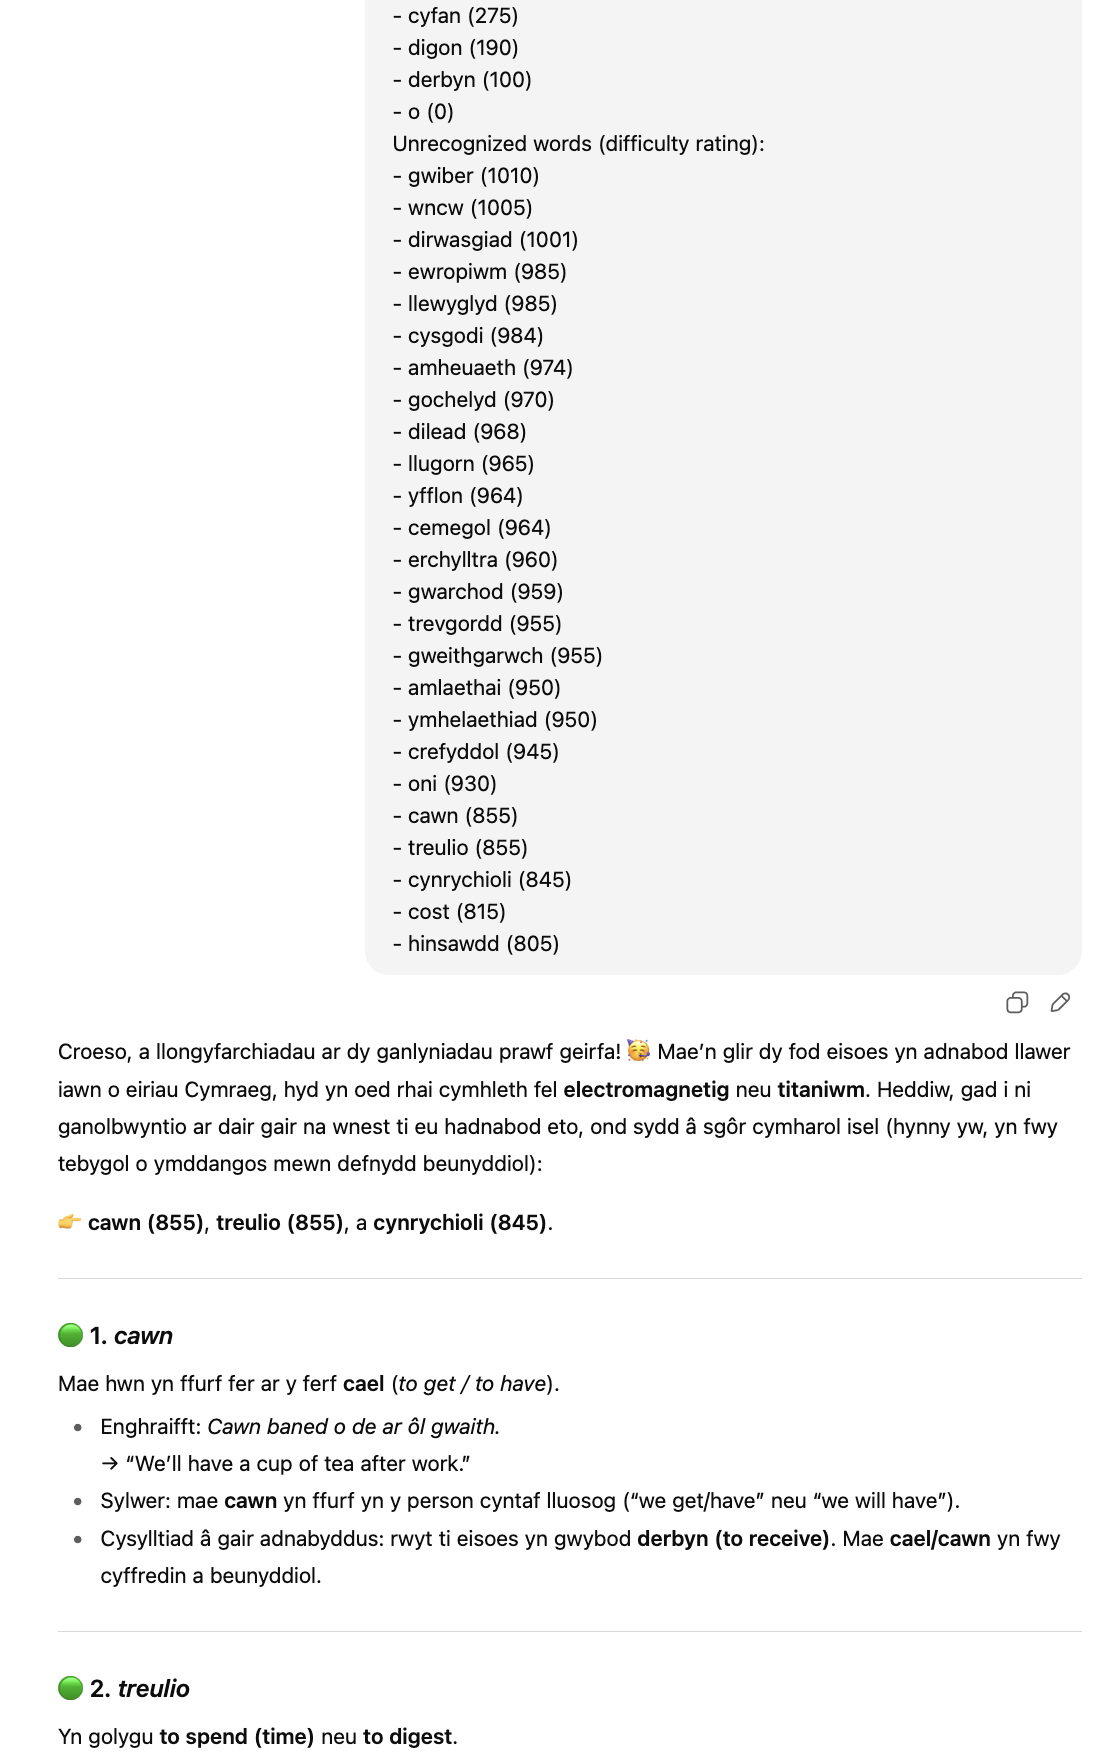
\includegraphics[width=0.8\textwidth]{figures/lesson-1.png}
    \caption{Beginning of a personalized lesson 1/2}
    \label{fig:lesson1}
\end{figure}
\begin{figure}[h]
    \centering
    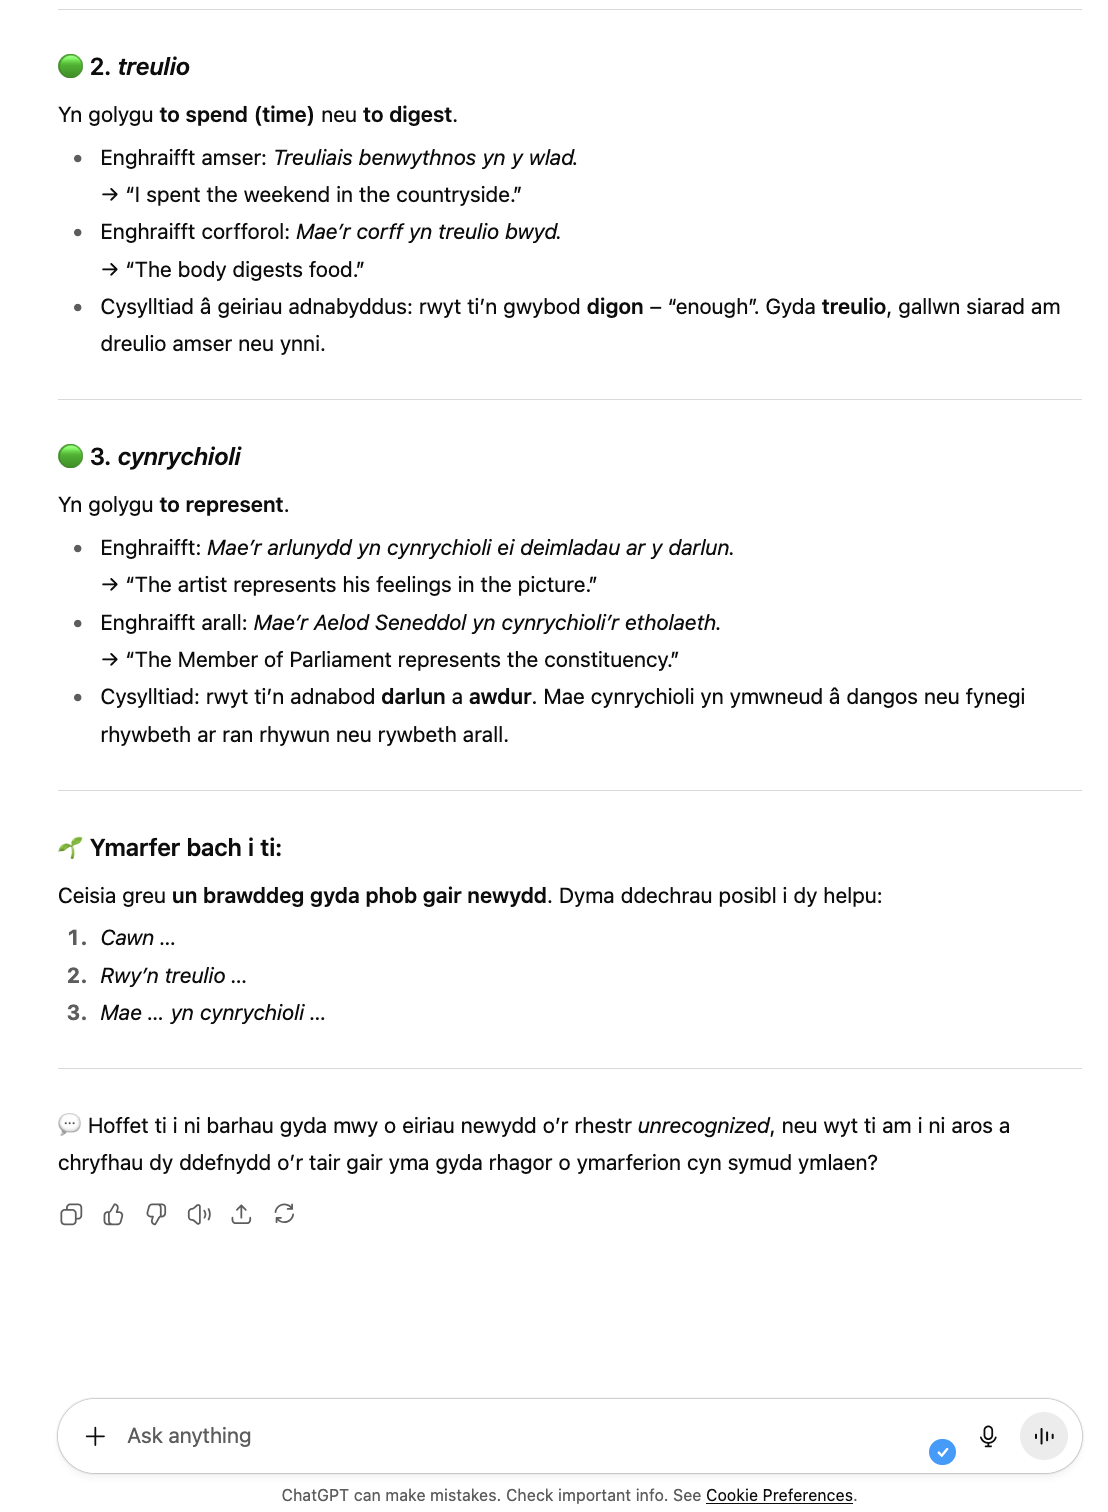
\includegraphics[width=0.8\textwidth]{figures/lesson-2.png}
    \caption{Beginning of a personalized lesson 2/2}
    \label{fig:lesson2}
    \medskip
    \small
    Indeed, ChatGPT can make mistakes, the word \textit{digon} is not mentioned anywhere, yet the second section implies it is present somewhere or that it is related in some way to the word \textit{treulio}. And \textit{gair} is masculine, so it should say \textit{tri gair} and not \textit{tair gair}. Interestingly however, the LLM seems to work out that the the lowest rated words proper, within the 800-850 rating range, may have been missed by mistake and start its lesson by the fourth to the sixth lowest rated unrecognised words.
\end{figure}

    \end{appendices}

    \printbibliography[title={Llyfryddiaeth}, heading=bibintoc]
\end{document}